\chapter{Supplemental Figures}

\begin{figure}
    \centering
    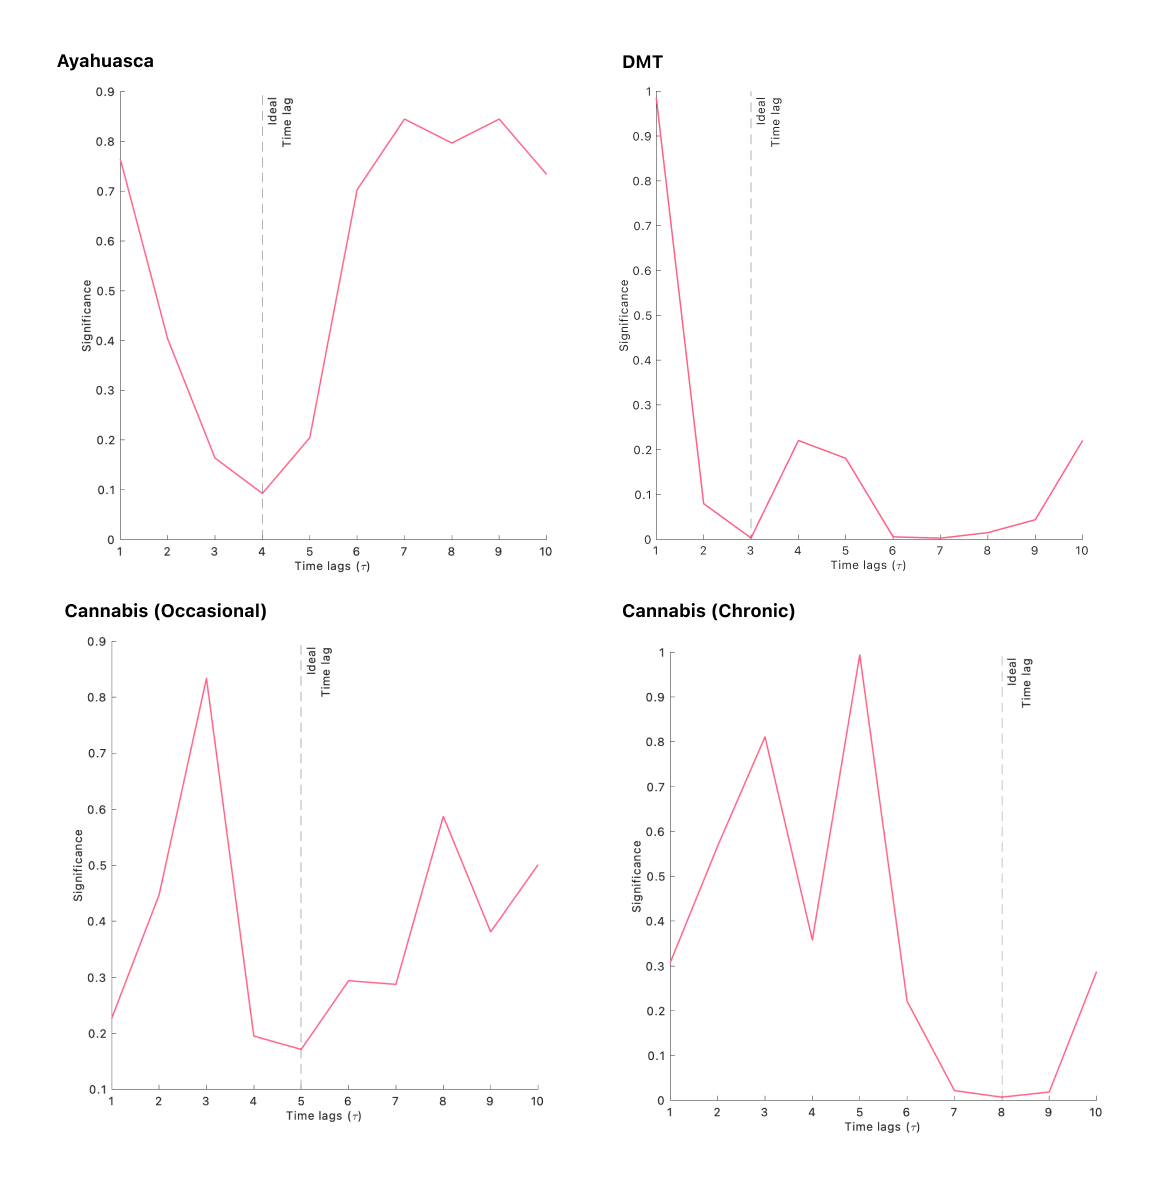
\includegraphics[width=\textwidth]{images/Appendix_ Tau Calculation.png}
    \caption[Establishing ideal $\tau$ for each condition.]{Evaluation of the ideal time-delay constant $\tau$ for each condition. Model-free irreversibility was calculated for Tau values 1 through 10 for each condition. For ayahuasca, occasional and chronic use of cannabis, a Wilcoxon rank-sum test was used to evaluate significance. The ideal Tau was determined as the most sensitive measure which best discriminates between baseline or placebo and drug conditions. For DMT, a mixed effects model was used in order to account for the pre-injection data as a covariate.}
    \label{fig:tau}
\end{figure}

\begin{figure}[h!]
    \centering
    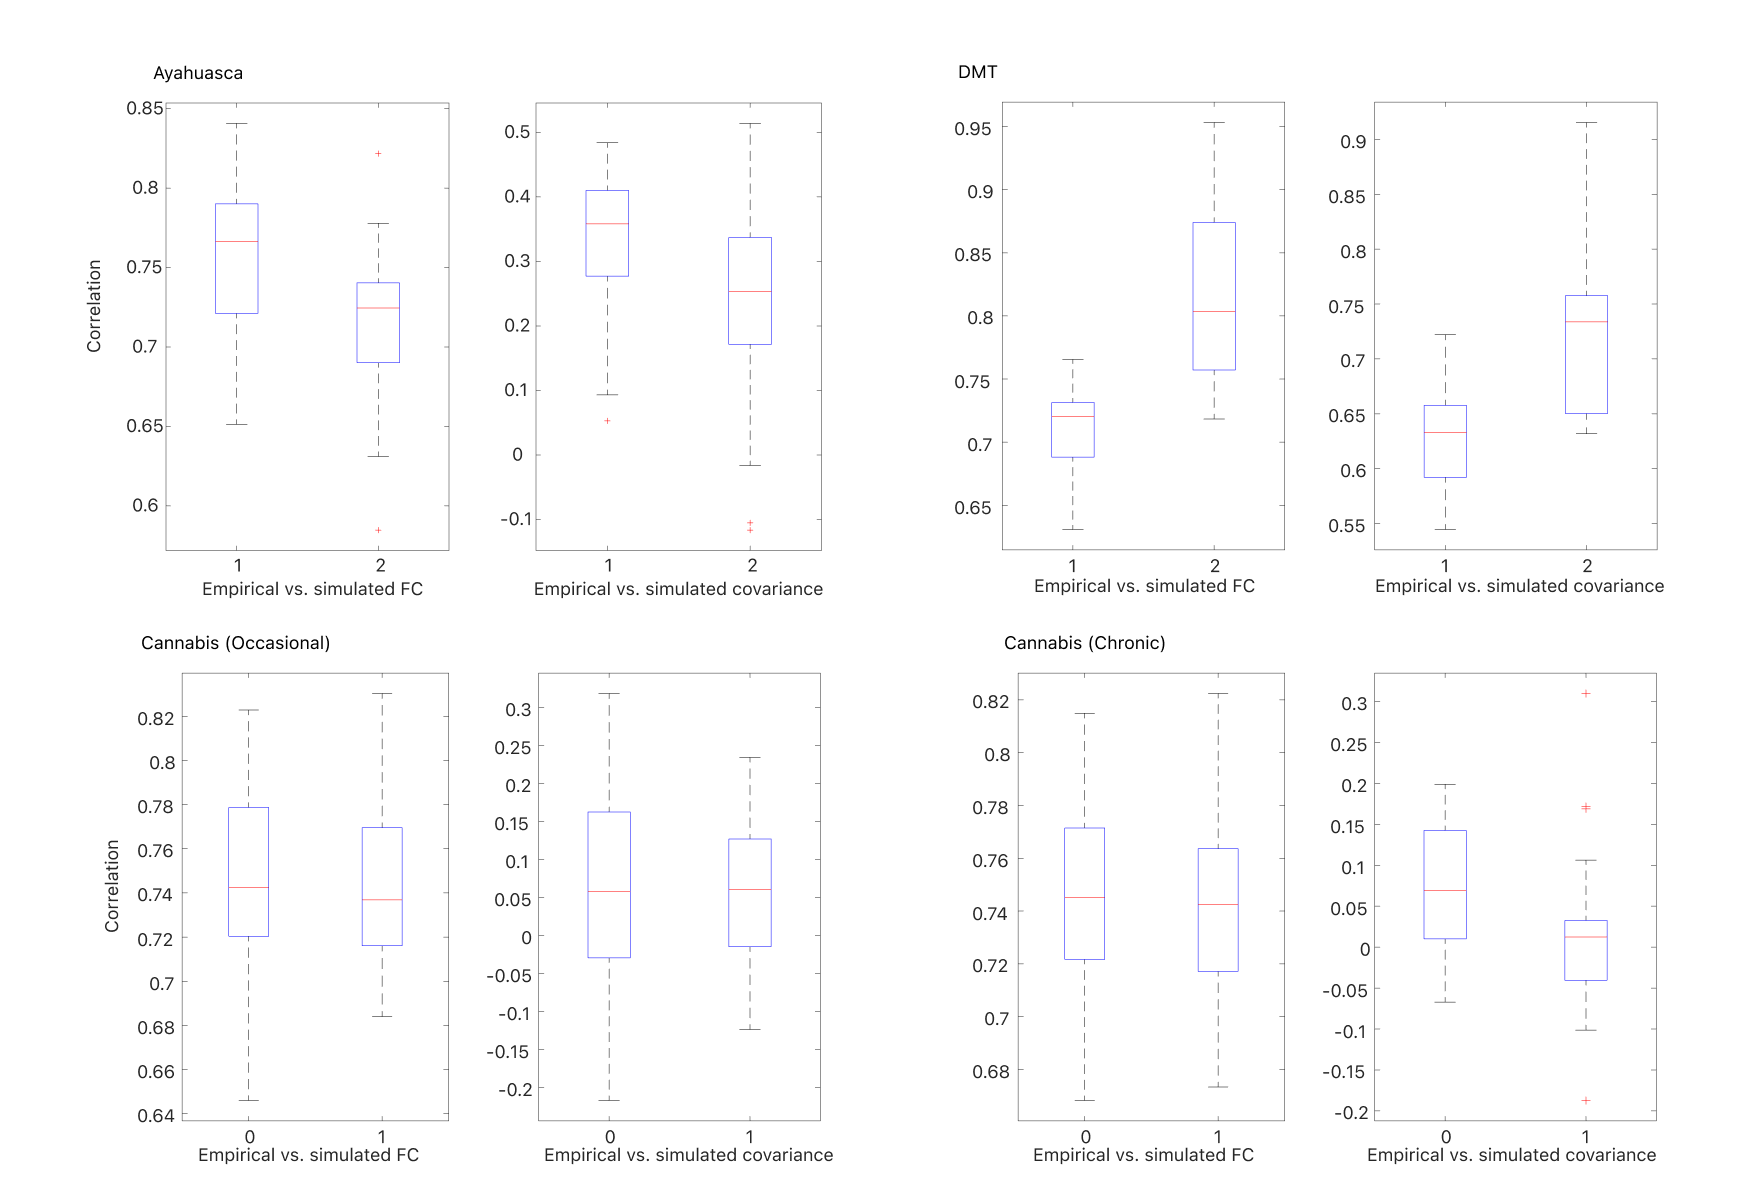
\includegraphics[width=\textwidth]{images/Appendix_ Fits.png}
    \caption[Whole-brain model fit.]{Correlations between empirical and simulated functional connectivity (left panel, each condition), and between empirical and simulated covariance of irreversibility matrices (right panel, each condition). "1" indicates baseline or placebo condition. "2" indicates drug condition.}
    \label{fig:fits}
\end{figure}

\begin{figure}[h!]
    \centering
    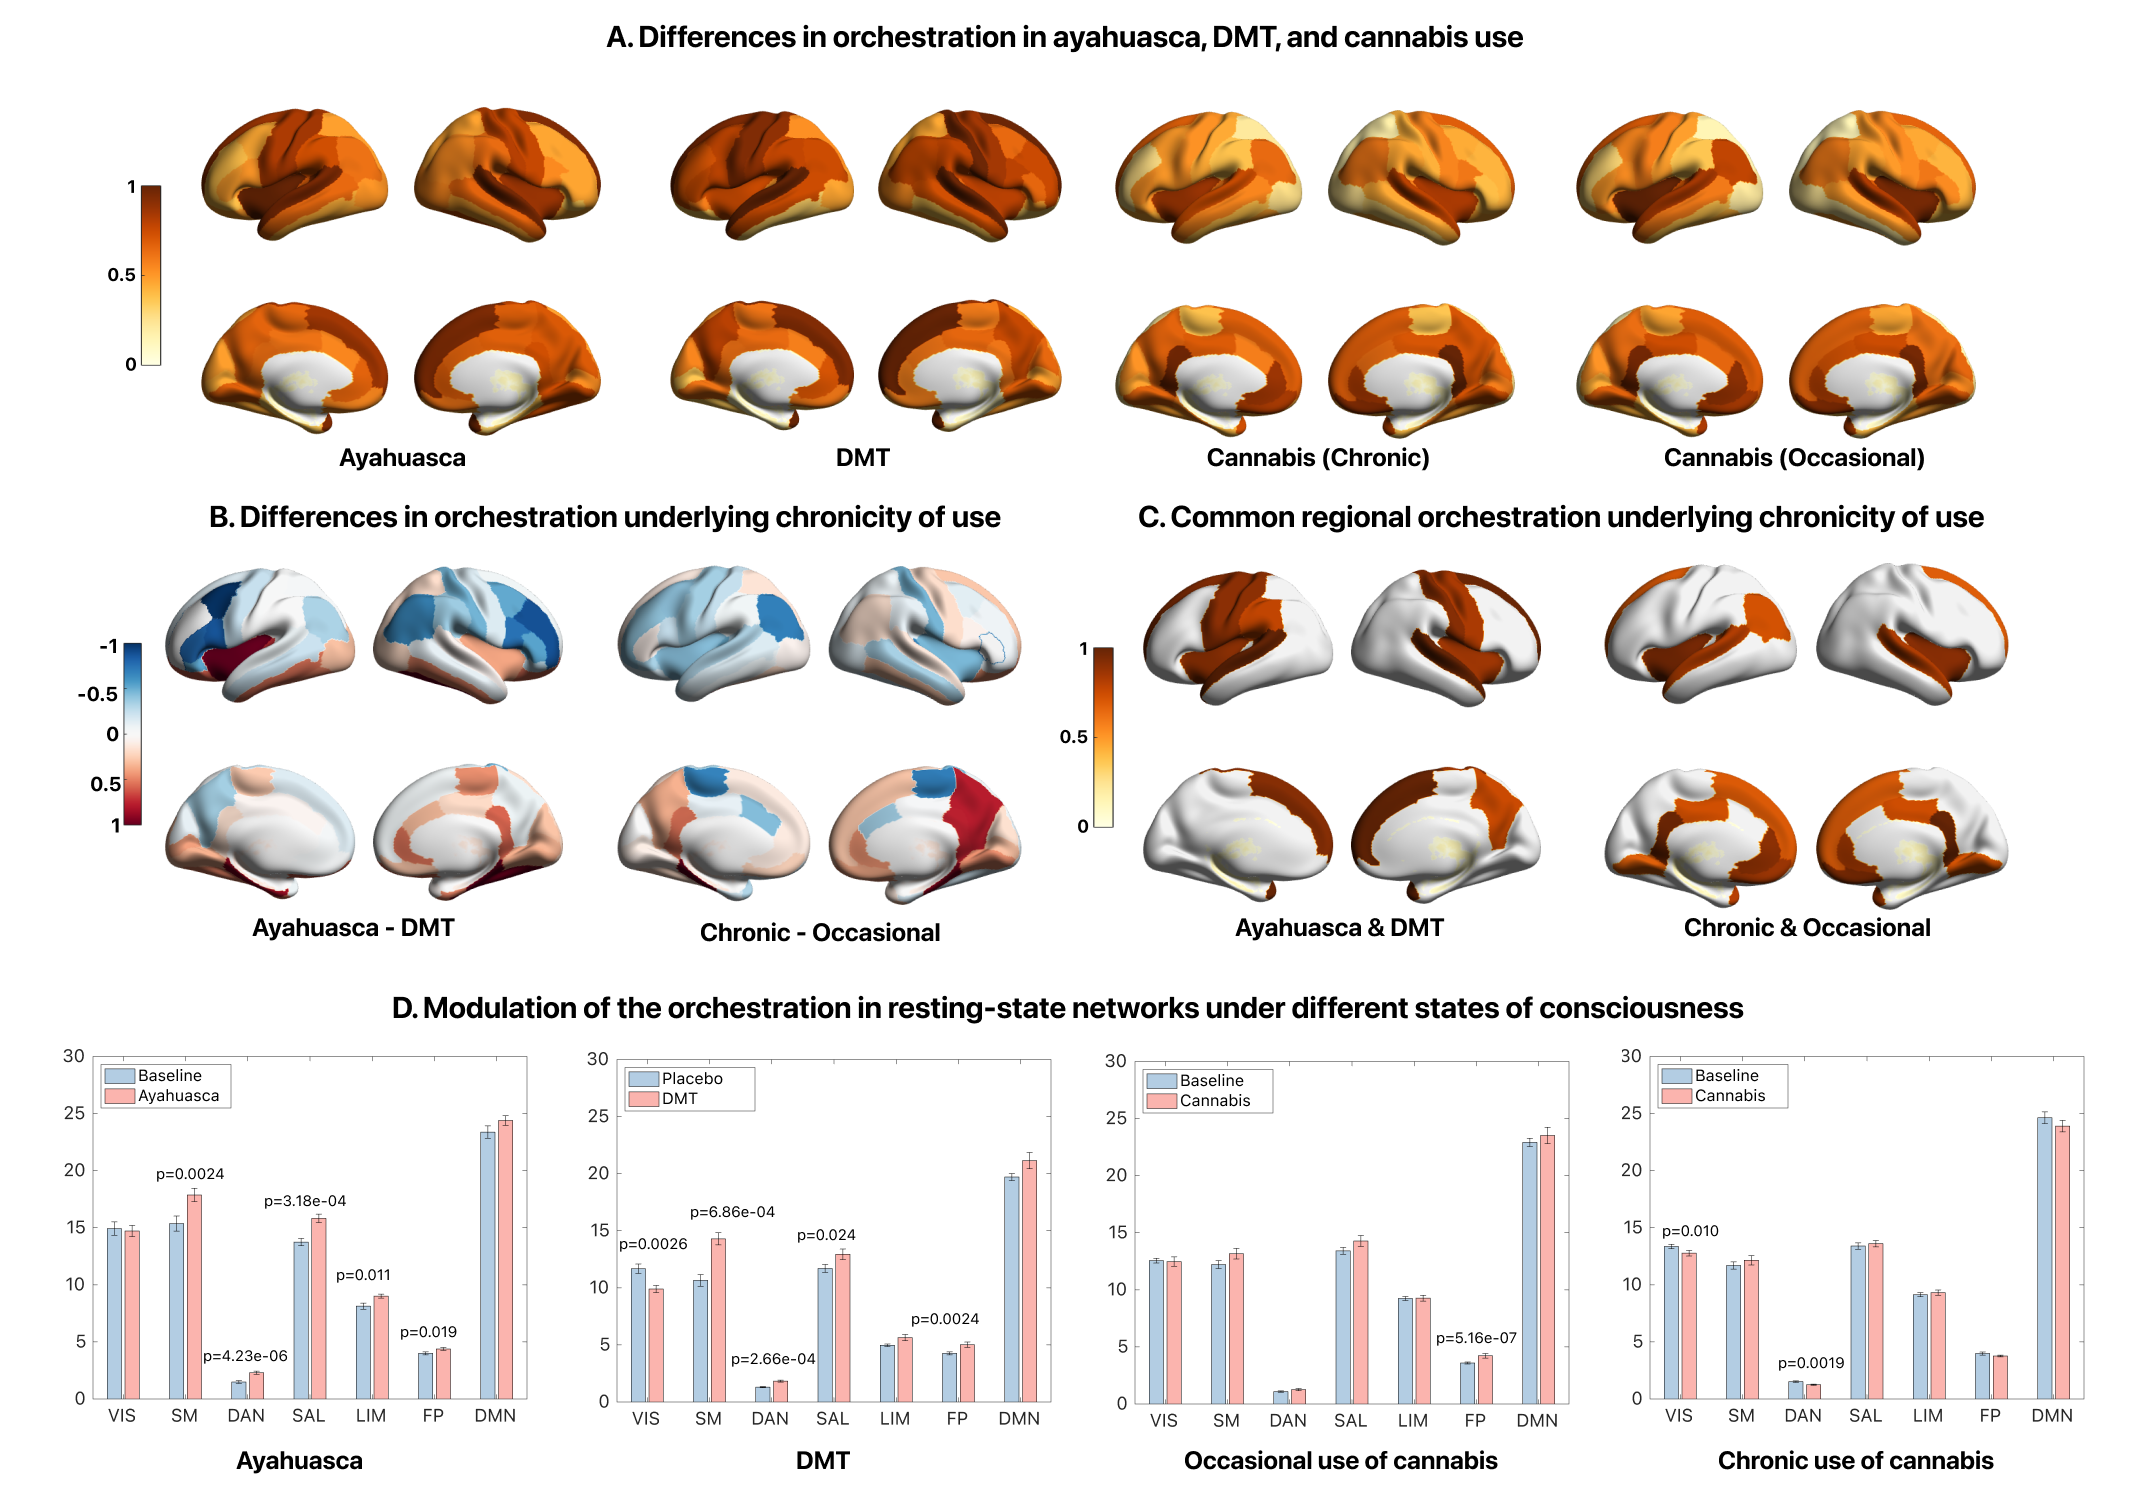
\includegraphics[width=\textwidth]{images/Appendix_GEC.png}
    \caption[Changes in directed connectivity in the psychedelic and cannabis states]{Differences in orchestration, a measure of total directed connectivity, under psychedelics and cannabis. (A) Measure of orchestration for each drug condition. Significant orchestrators for ayahuasca and DMT include bilateral pre- and post-central, insula, and superior frontal. For cannabis, bilateral insula, isthmus cingulate, and caudal anterior cingulate were found to be more connected than other regions in the brain. (B) Differences in orchestration between psychedelics, ayahuasca and DMT, and chronic and occasional use of cannabis. (C) Common orchestrators under psychedelics and cannabis. (D) Modulation of network-level orchestration under psychedelics and cannabis. Non-parametric permutation testing (5,000 iterations, threshold = 0.01) was utilized to evaluate changes in individual resting-state networks for each drug condition.}
    \label{fig:gecrender}
\end{figure}
\begin{figure}[h!]
    \centering
    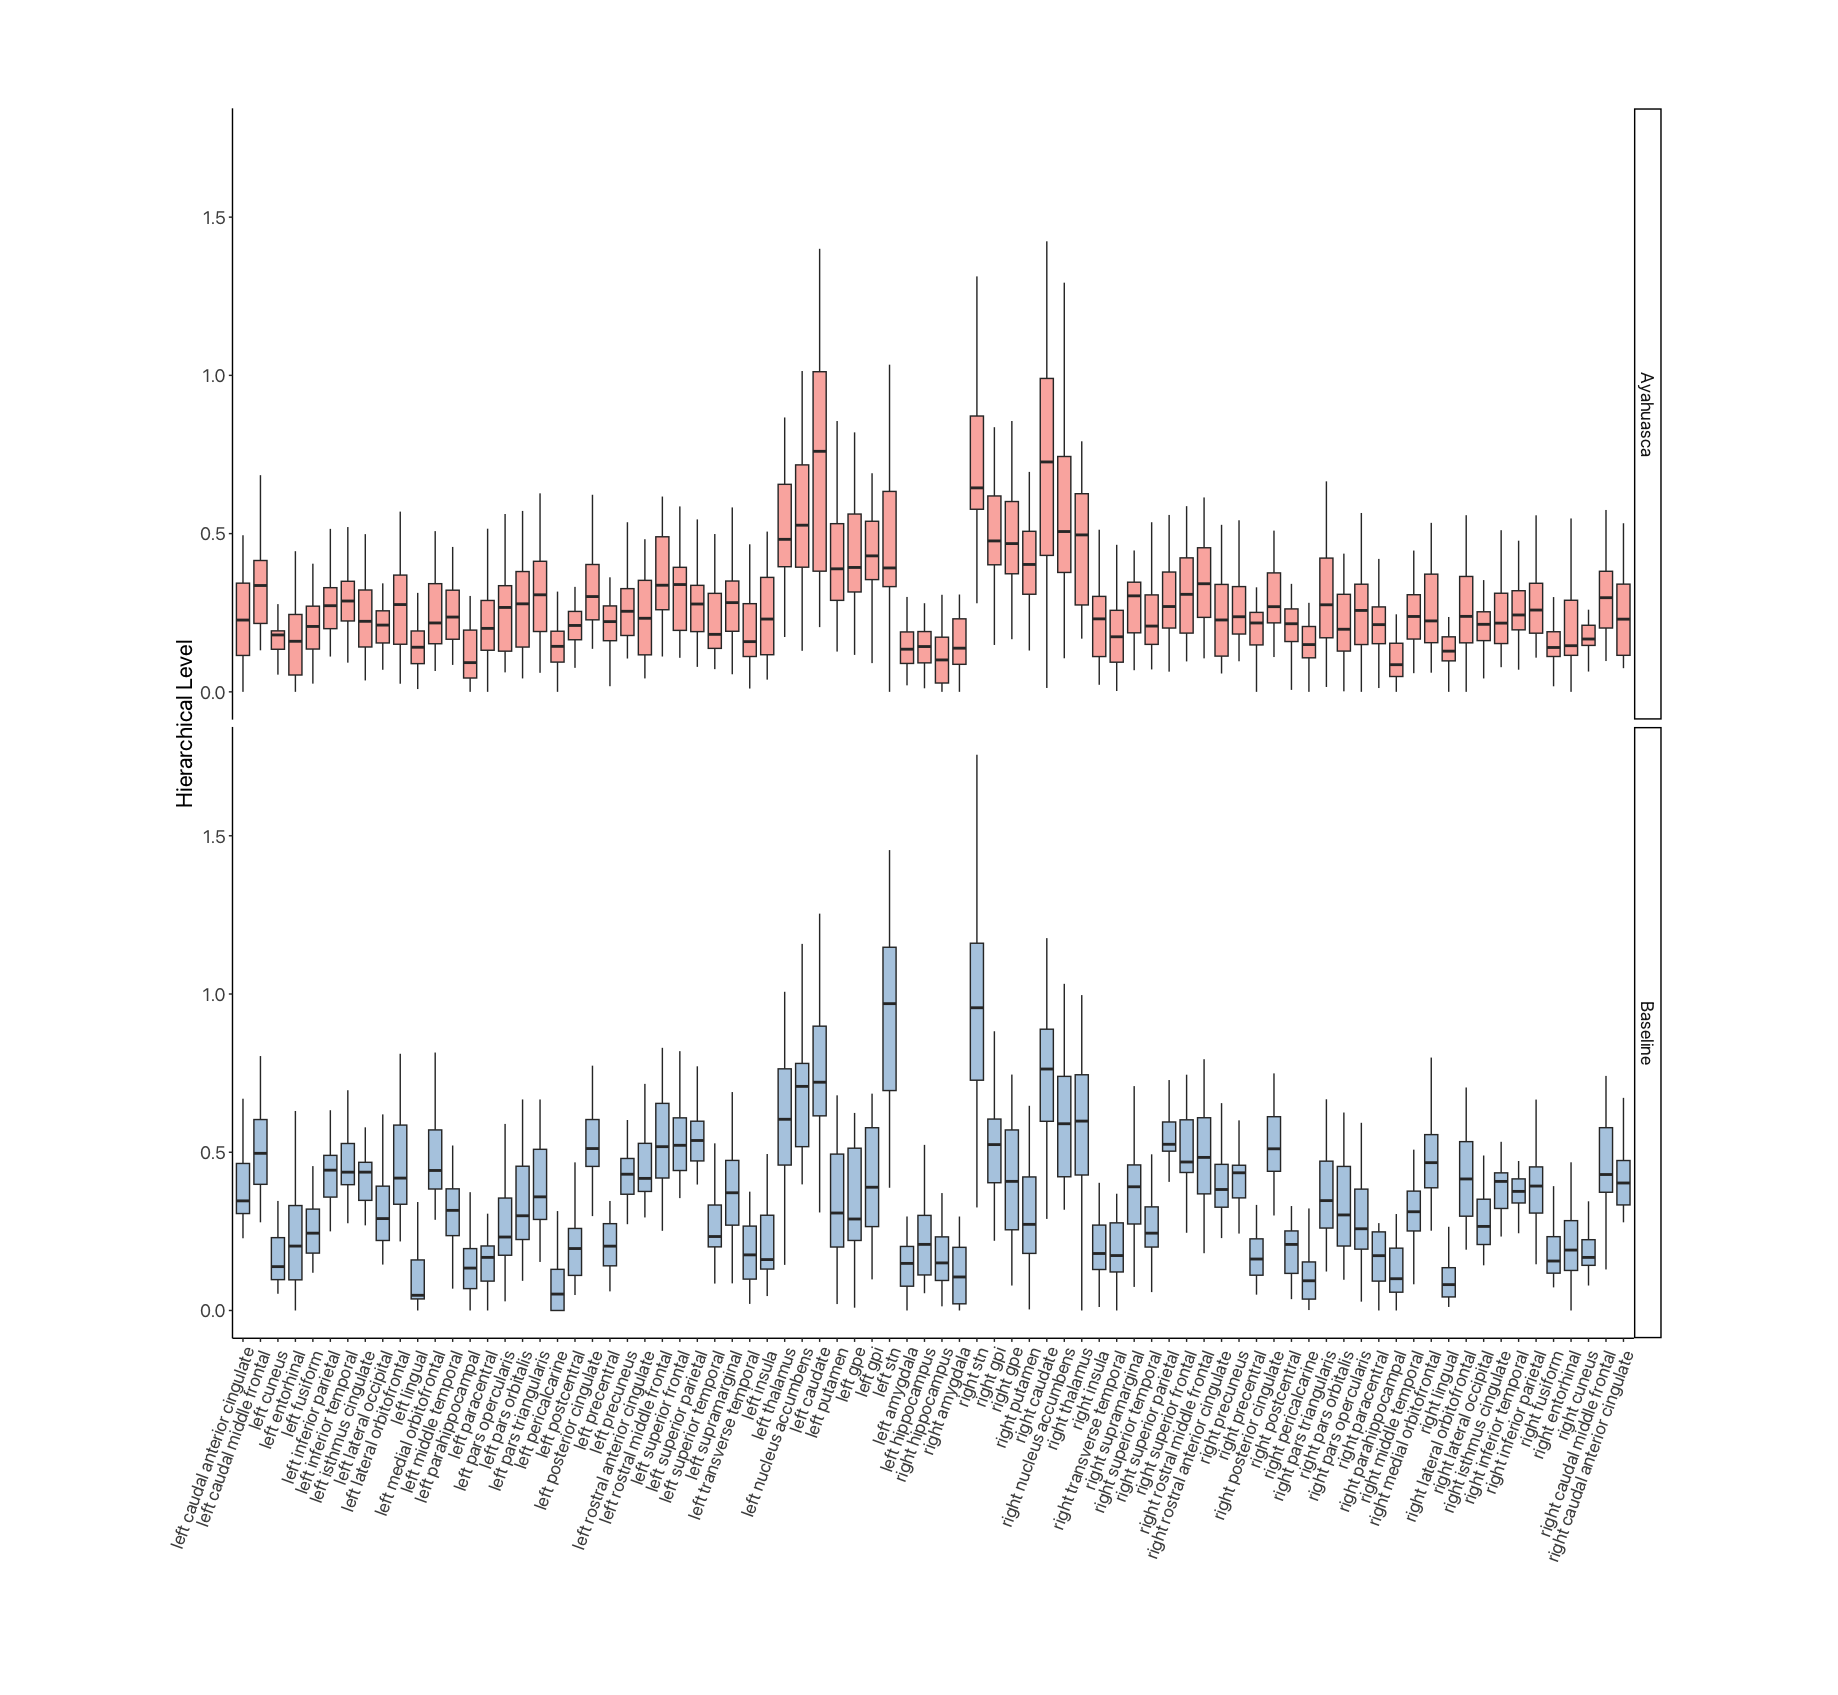
\includegraphics[width=\textwidth]{images/Appendix_ AYA HL.png}
    \caption[Regional hierarchical levels under baseline and ayahuasca.]{Hierarchical levels for each region in the DBS80 across baseline and ayahuasca conditions. Top panel, ayahuasca. Bottom panel, baseline.}
    \label{fig:ayahl}
\end{figure}

\begin{figure}[h!]
    \centering
    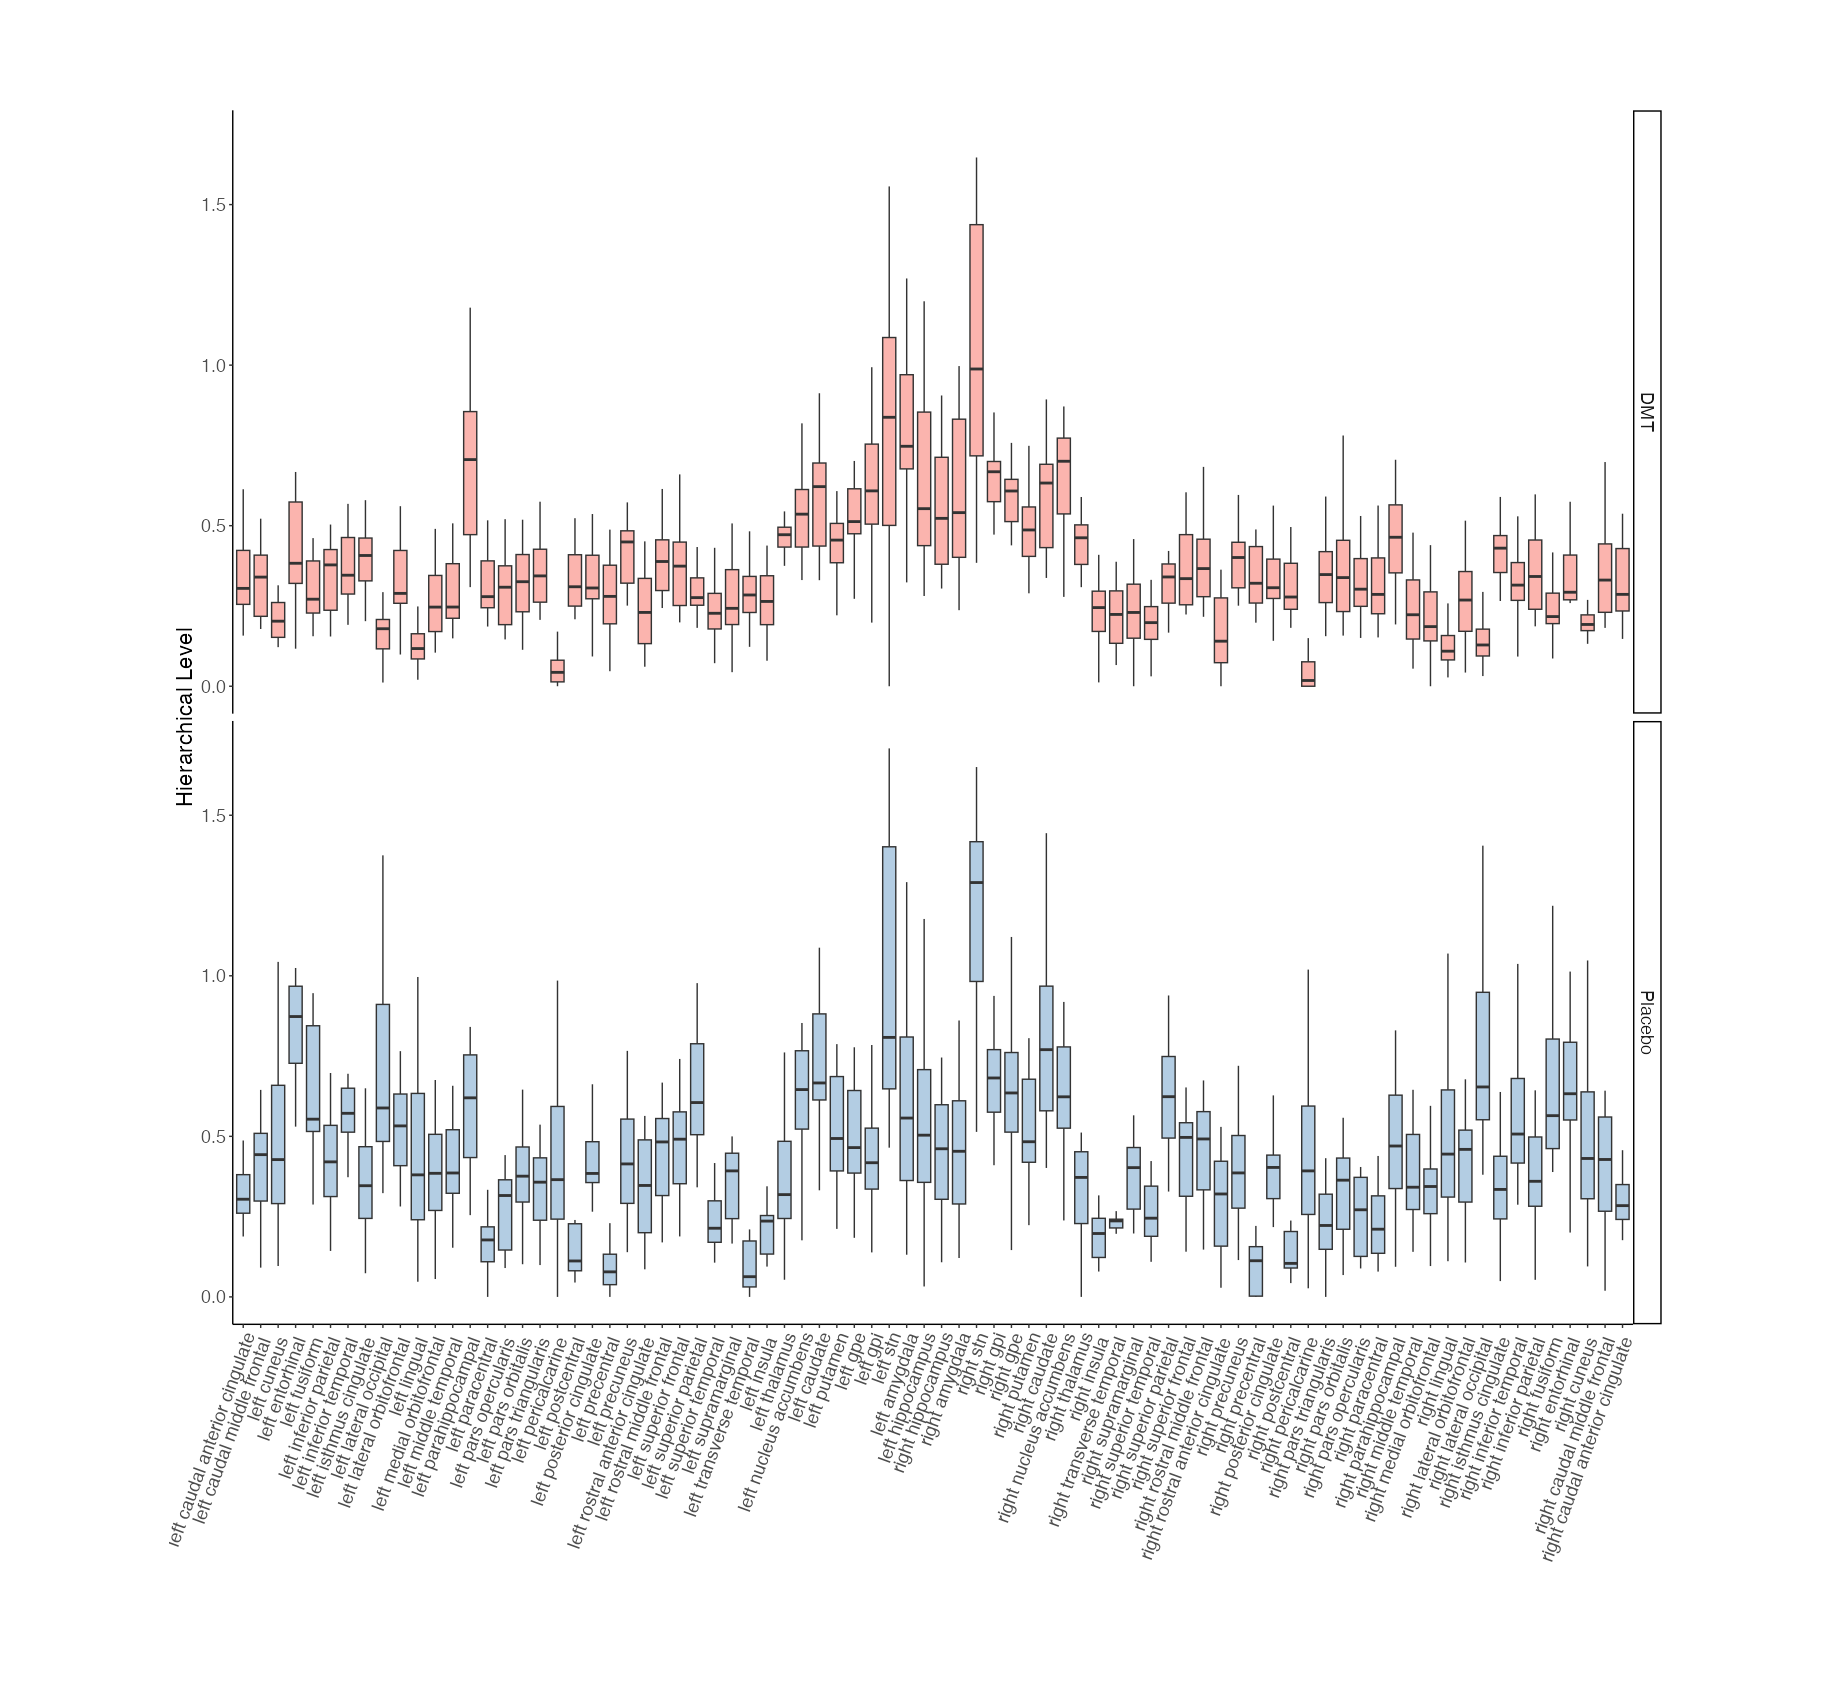
\includegraphics[width=\textwidth]{images/Appendix_ DMT HL.png}
    \caption[Hierarchical levels under placebo and DMT.]{Hierarchical levels for each region in the DBS80 across placebo and DMT conditions. Top panel, DMT. Bottom panel, placebo.}
    \label{fig:dmthl}
\end{figure}

\begin{figure}[h!]
    \centering
    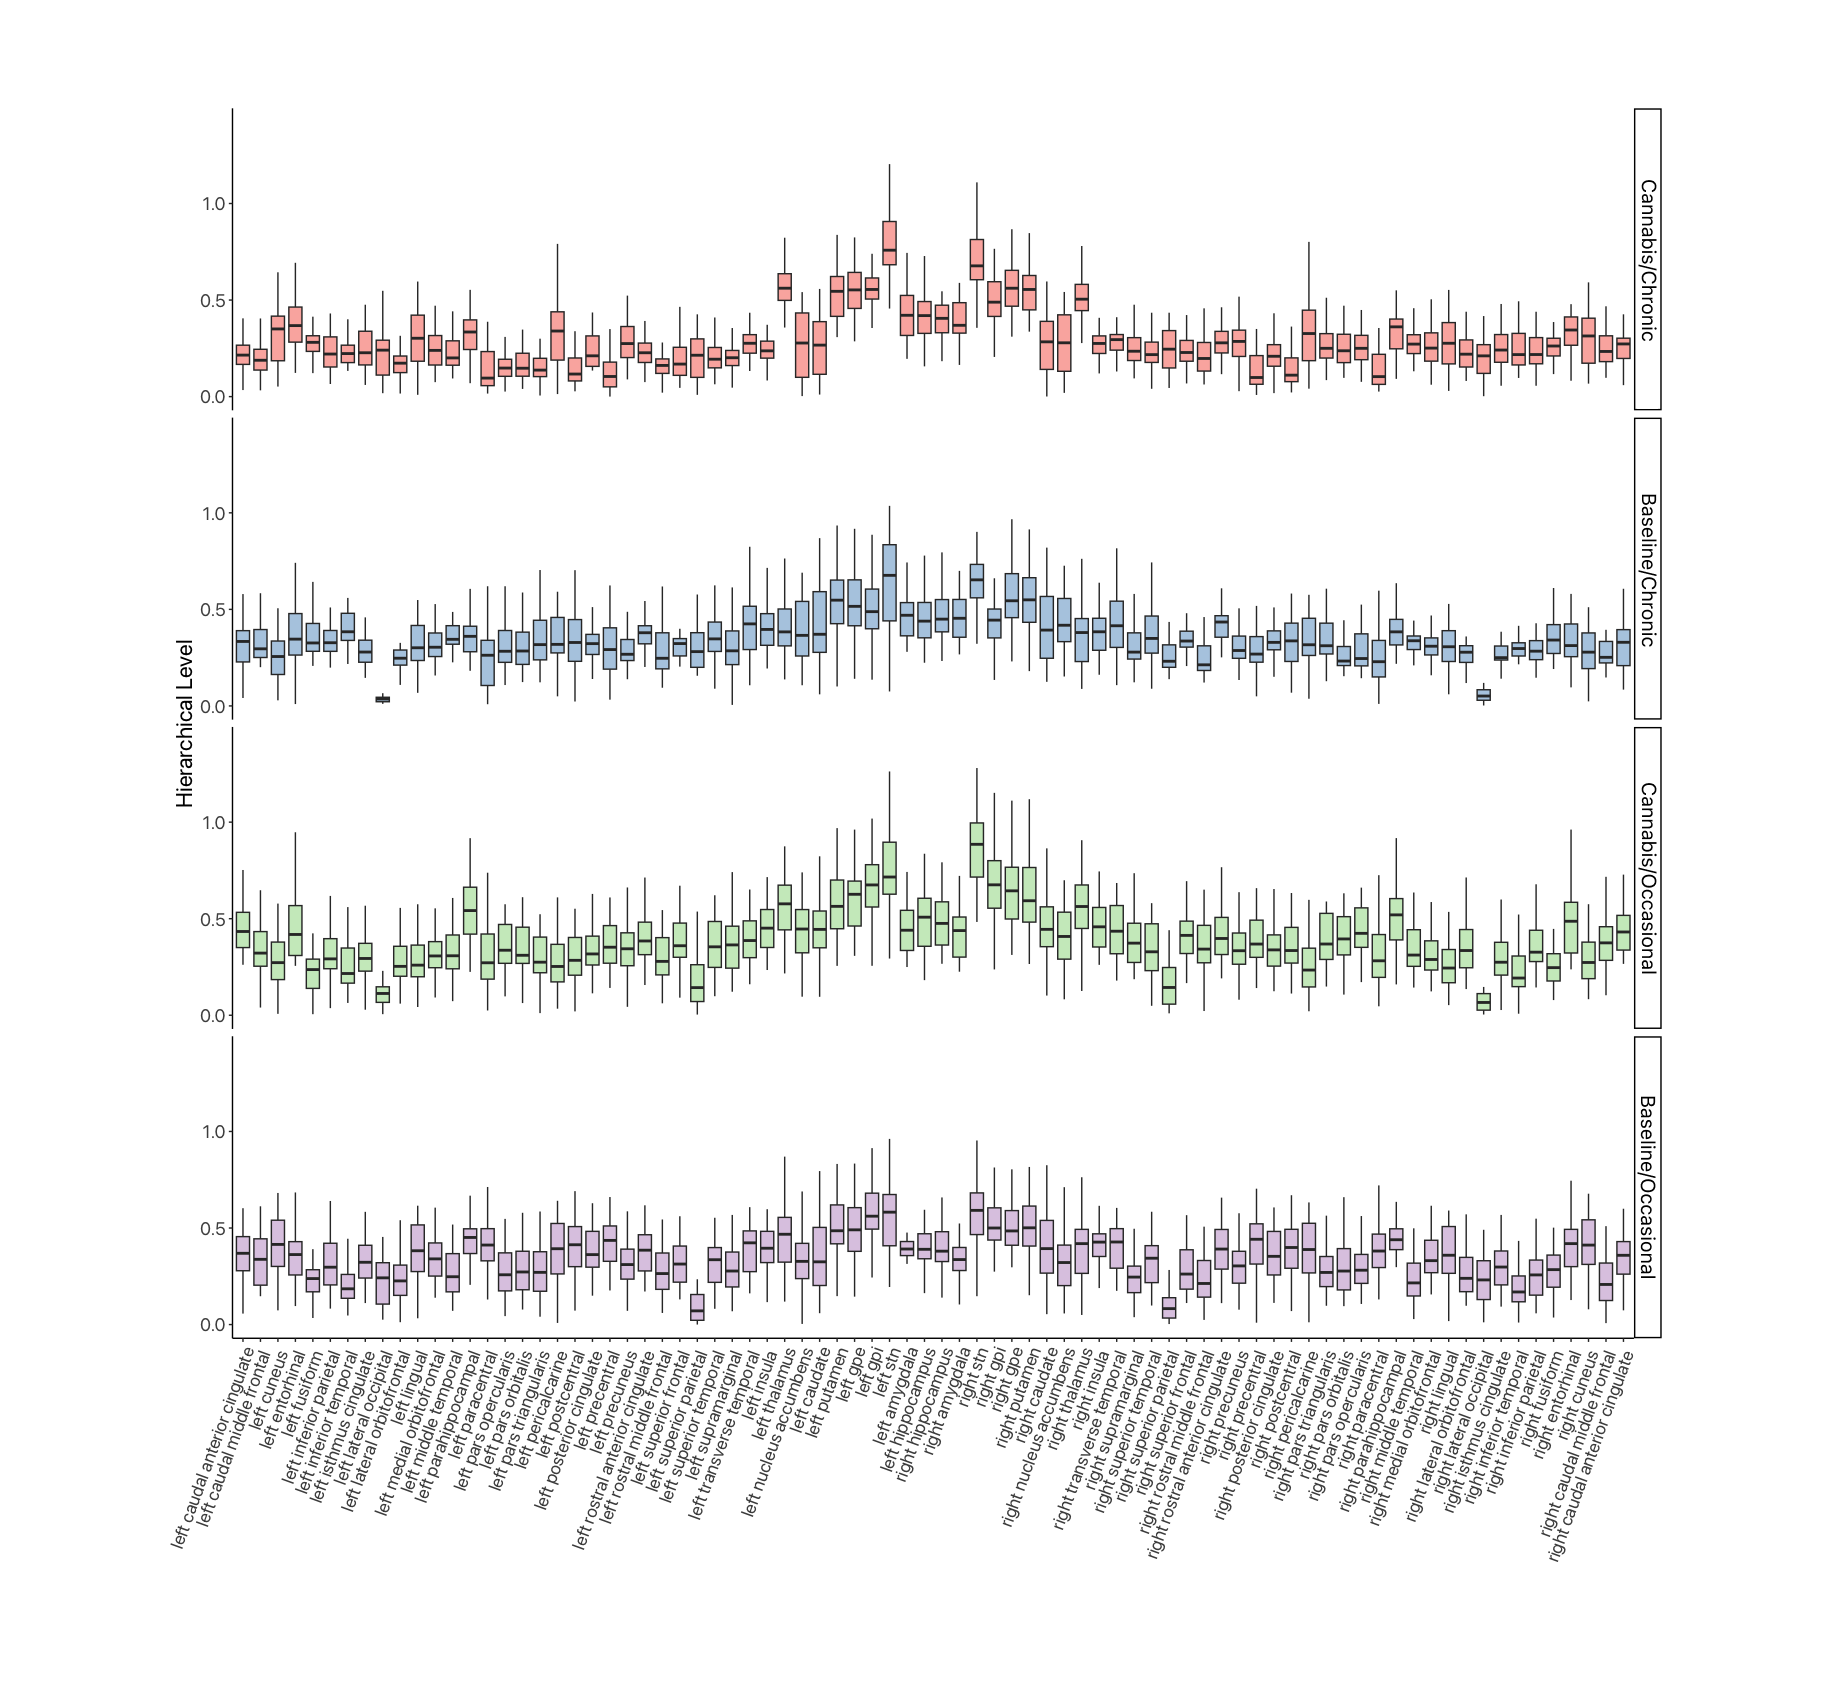
\includegraphics[width=\textwidth]{images/Appendix_ Cannab HL.png}
    \caption[Hierarchical levels under baseline and cannabis in chronic and occasional users.]{Hierarchical levels for each region in the DBS80 across baseline and cannabis (both chronic and occasional users). Top panel, cannabis in chronic users. Mid-top panel, baseline in chronic users. Mid-bottom panel, cannabis in occasional users. Bottom panel, baseline in occasional users.}
    \label{fig:cannabishl}
\end{figure}